\documentclass{article}

\usepackage{microtype}
\usepackage{graphicx}
\usepackage{subfigure}
\usepackage{booktabs} % for professional tables


\usepackage{hyperref}

% Attempt to make hyperref and algorithmic work together better:
\newcommand{\theHalgorithm}{\arabic{algorithm}}


\usepackage[accepted]{icml2021}

% The \icmltitle you define below is probably too long as a header.
% Therefore, a short form for the running title is supplied here:
\icmltitlerunning{Image Animation with Keypoint Mask}

\begin{document}

\twocolumn[
\icmltitle{Image Animation with Keypoint Mask}

\icmlsetsymbol{equal}{*}

\begin{icmlauthorlist}
\icmlauthor{Or Toledano}{tlv}
\icmlauthor{Yanir Marmor}{tlv}
\icmlauthor{Dov Gertz}{tlv}

\end{icmlauthorlist}

\icmlaffiliation{tlv}{Tel Aviv University}

\icmlcorrespondingauthor{Or Toledano}{ortoledano@protonmail.com}

\icmlkeywords{Machine Learning, ICML}

\vskip 0.3in
]
\printAffiliationsAndNotice{}  % leave blank if no need to mention equal contribution
%\printAffiliationsAndNotice{\icmlEqualContribution} % otherwise use the standard text.

\begin{abstract}
TODO OR
important
transgaga structure
realtime
\cite{siarohin2020order}
\end{abstract}

\section{Introduction}
TODO Or

Our paper focuses on the motion transfer problem: given a source image $S$
and a driving video $D$, the goal is to syntesize a video with the identity
of $S$, and the motion from $D$.
Some notable works \cite{siarohin2020order}, \cite{wiles2018x2face},
\cite{siarohin2019animating}.

Our method does not rely on GANs - see Section~\ref{method}.

\medskip

\textbf{Related Work:} Our work doesn't rely directly on a strong motion prior,
but uses a structure mask which was extracted from a keypoint detector
of a motion based model, such as \cite{siarohin2020order}. The concept of using drawn keypoints as
a geometry represantation (structural mask) was already used in the context
of image-to-image translation, in works such as TransGaGa \cite{wu2019transgaga}.
The concept of using a structural mask in the context of image animation is
demonstrated in \cite{shalev2020image}. However, the current work differs
by basing the mask off a motion related module, which saves us the hassle
of perturbing the input hoping to achieve an identy-less mask. By doing so,
we improve their results, and purposes an additional "circles" only mask
which can be used in the context
of relative motion transfer during animation, as in
\cite{siarohin2020order}, which isn't possible with a mask.

\section{Methodology}
Methods
methods
methods
\label{method}
\begin{figure}[ht]
\vskip 0.2in
\begin{center}
\centerline{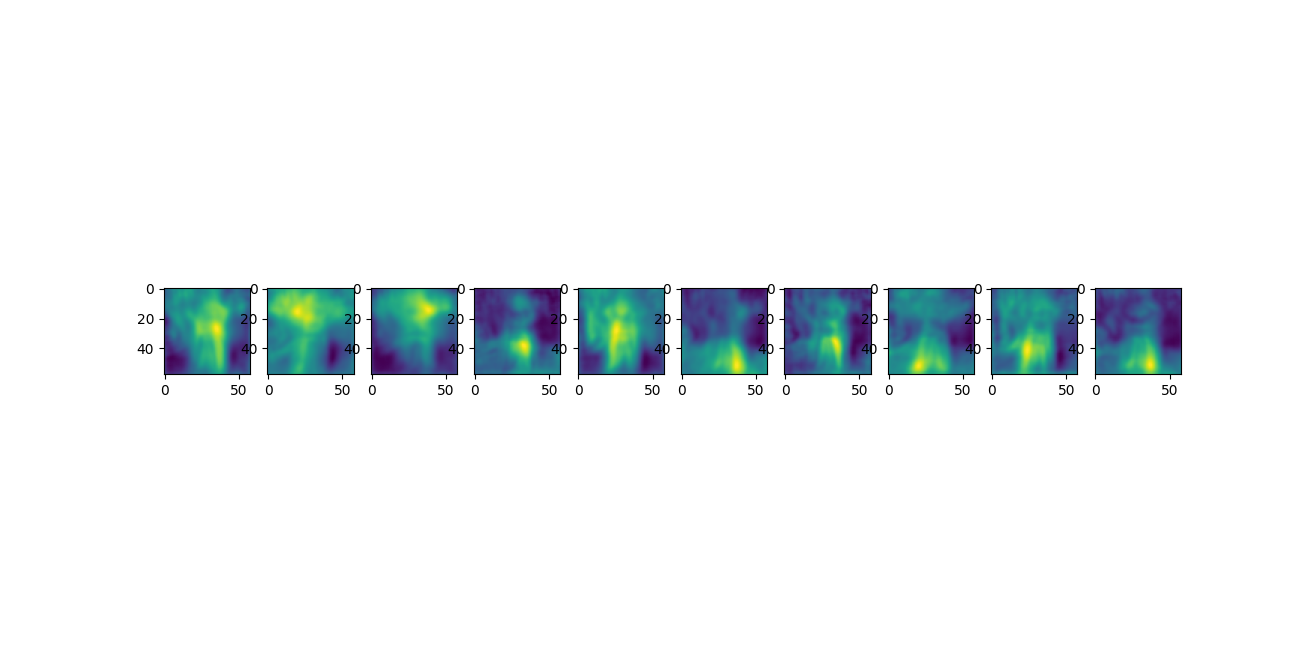
\includegraphics[width=\columnwidth]{mask_10kp}}
\caption{
$K$ channels of the keypoint detector network used in
\cite{siarohin2020order}, before the softmax activation. Our main motion
prior in this project.
}
\label{mask-10kp}
\end{center}
\vskip -0.2in
\end{figure}
\section{Experiments}


TODO Yanir/Dov
\\
TODO like fomm/yoav
TODO video reconstructioncomparison like yoav/fomm

\begin{tabular}{m{1.5cm}m{1.5cm}m{1.5cm}}
\toprule
 Source image & Driving\\
\toprule
 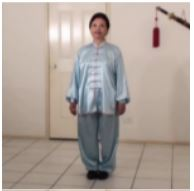
\includegraphics[width=1cm, height=1cm]{paper/images/source.JPG}& 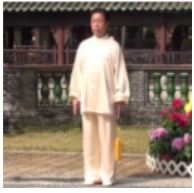
\includegraphics[width=1cm, height=1cm]{paper/images/driving1.JPG} & 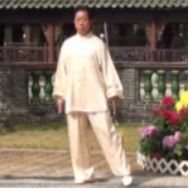
\includegraphics[width=1cm, height=1cm]{paper/images/driving2.JPG} & 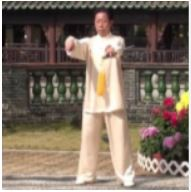
\includegraphics[width=1cm, height=1cm]{paper/images/driving3.JPG} & 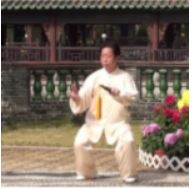
\includegraphics[width=1cm, height=1cm]{paper/images/driving4.JPG}&
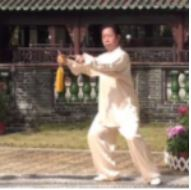
\includegraphics[width=1cm, height=1cm]{paper/images/driving5.JPG}\\
\midrule
X2Face & 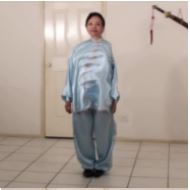
\includegraphics[width=1cm, height=1cm]{paper/images/1_X2Face_1.JPG} & 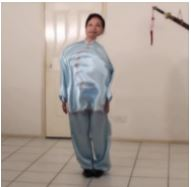
\includegraphics[width=1cm, height=1cm]{paper/images/1_X2Face_2.JPG} &
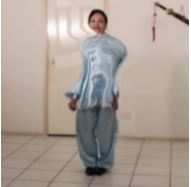
\includegraphics[width=1cm, height=1cm]{paper/images/1_X2Face_3.JPG}&
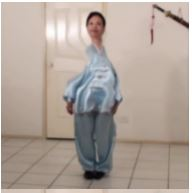
\includegraphics[width=1cm, height=1cm]{paper/images/1_X2Face_4.JPG}&
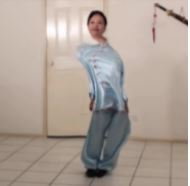
\includegraphics[width=1cm, height=1cm]{paper/images/1_X2Face_5.JPG}\\
Monkey-Net & 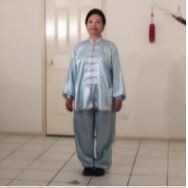
\includegraphics[width=1cm, height=1cm]{paper/images/2_Monkey-Net_1.JPG} & 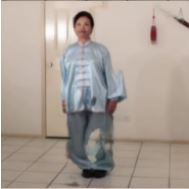
\includegraphics[width=1cm, height=1cm]{paper/images/2_Monkey-Net_2.JPG} &
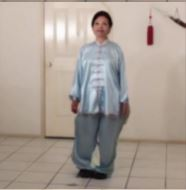
\includegraphics[width=1cm, height=1cm]{paper/images/2_Monkey-Net_3.JPG}&
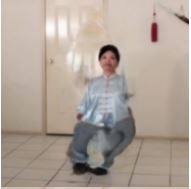
\includegraphics[width=1cm, height=1cm]{paper/images/2_Monkey-Net_4.JPG}&
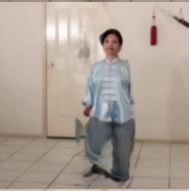
\includegraphics[width=1cm, height=1cm]{paper/images/2_Monkey-Net_5.JPG}\\
FOMM & 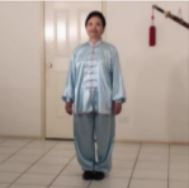
\includegraphics[width=1cm, height=1cm]{paper/images/3_FOMM_1.JPG} & 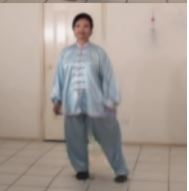
\includegraphics[width=1cm, height=1cm]{paper/images/3_FOMM_2.JPG} &
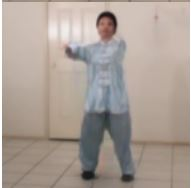
\includegraphics[width=1cm, height=1cm]{paper/images/3_FOMM_3.JPG}&
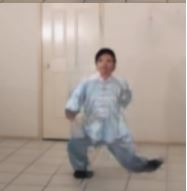
\includegraphics[width=1cm, height=1cm]{paper/images/3_FOMM_4.JPG}&
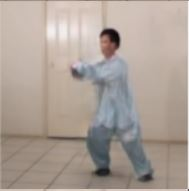
\includegraphics[width=1cm, height=1cm]{paper/images/3_FOMM_5.JPG}\\
YOAV & 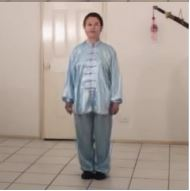
\includegraphics[width=1cm, height=1cm]{paper/images/4_YOAV_1.JPG} & 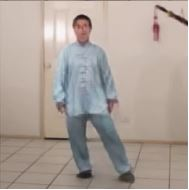
\includegraphics[width=1cm, height=1cm]{paper/images/4_YOAV_2.JPG} &
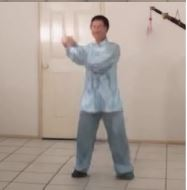
\includegraphics[width=1cm, height=1cm]{paper/images/4_YOAV_3.JPG}&
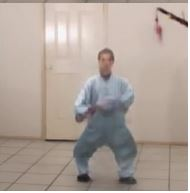
\includegraphics[width=1cm, height=1cm]{paper/images/4_YOAV_4.JPG}&
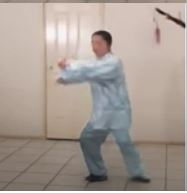
\includegraphics[width=1cm, height=1cm]{paper/images/4_YOAV_5.JPG}\\
\bottomrule
\end{tabular}




\subsection{Datasets}
TODO
\subsection{Comparison with Previous Works}
We can see:
\label{results}
TODO Dov
% Note use of \abovespace and \belowspace to get reasonable spacing
% above and below tabular lines.

\begin{table}[t]
\caption{Accuracy Metrics}
\label{sample-table}
\vskip 0.15in
\begin{center}
\begin{small}
\begin{sc}
\begin{tabular}{lcccr}
\toprule
Method & AKD & AED & L1 \\
\midrule
Monkey-Net    & 10.798 & 0.228 & 0.077 \\
FOMM    & 6.872 & 0.167 & 0.063 \\
Yoav & 4.239 & 0.147 & 0.047 \\
Ours softmax & 14.760& 0.245 & $\times$ \\
Ours & 5.551 & 0.141 &  0.045\\
\midrule
Improvement (FOMM)    & 19.2\% & 15.5\% & 28.5\% \\
\bottomrule
\end{tabular}
\end{sc}
\end{small}
\end{center}
\vskip -0.1in
\end{table}

\section*{Software and Data}
Detailed in our repository:
{\footnotesize
\url{https://github.com/or-toledano/animation-with-keypoint-mask}
}

\bibliography{animation-with-keypoint-mask}
\bibliographystyle{icml2021}

\end{document}
